\begin{figure}[htbp]
\centering
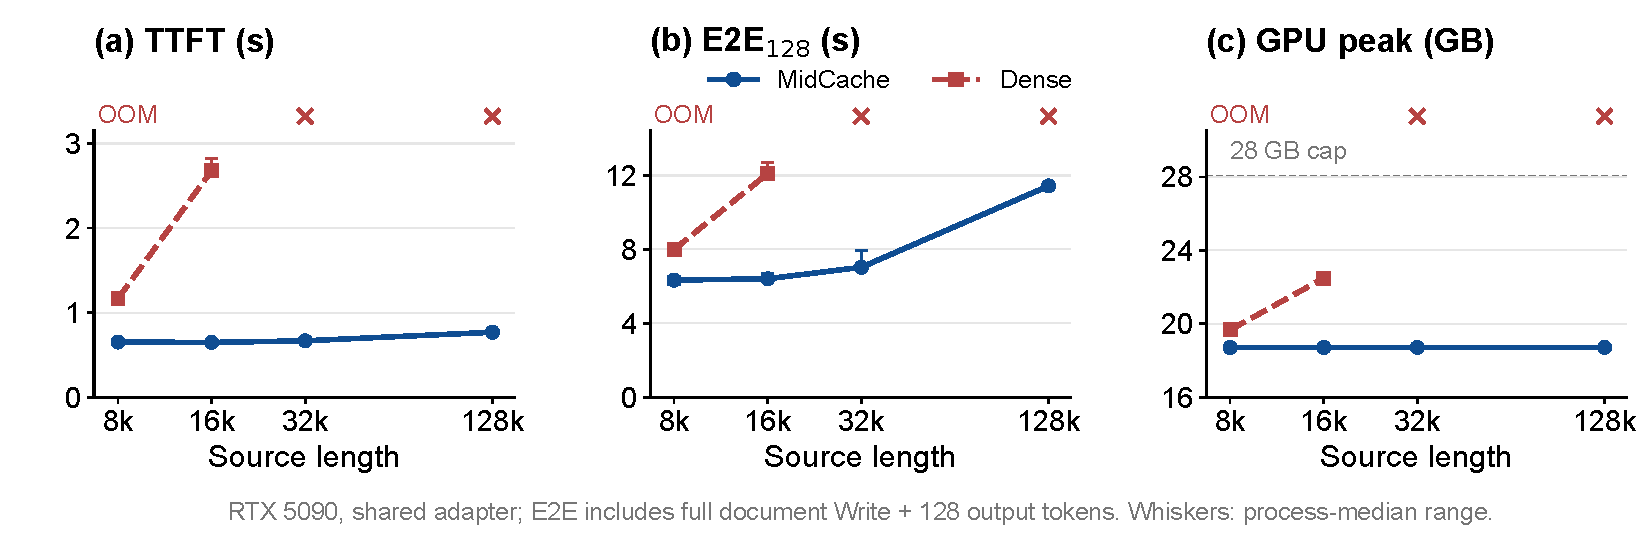
\includegraphics[width=\linewidth]{figures/source_scaling.pdf}
\caption{\textbf{Source-length scaling on RTX 5090.} These are the Table~\ref{tab:infra}(a) measurements with a shared adapter and three documents per length. Source length uses a base-two logarithmic axis. Latency markers are medians of three process medians; whiskers show their range, not a confidence interval. TTFT excludes document Write; E2E includes fresh document preparation and a fixed 128-token output. GPU values are maximum TTFT allocated peaks including weights. Red crosses above the axes mark Dense OOMs at 32k and 128k under the 28 GB allocator cap; they have no numerical ordinate. MidCache's 32k/128k measurements use a tighter 26 GB cap. Full inputs, repetition counts, and timing boundaries are specified in this appendix.}
\label{fig:source-scaling}
\end{figure}
